%% ============================================================

\clearpage
\section{Metric Details}
\label{app:metric-details}
%%%% Starting from Table 11 %%%%%%%%%
\begin{table}[h]
\centering
\small
\captionsetup{font=small}
\caption{\framework~metrics organized by category. All EVA-A and EVA-X 
scores are normalized to $[0,1]$ prior to aggregation. Thresholds are 
used for \passatk~and \passpowerk~computation: a run is considered 
successful if all EVA-A and EVA-X metrics meet their respective 
thresholds simultaneously.}
\begin{tabular}{lllll}
\toprule
\textbf{Category} & \textbf{Metric} & \textbf{Type} & 
\textbf{Scale} & \textbf{Pass Thresholds} \\
\midrule
\multirow{3}{*}{EVA-A (Accuracy)}
  & Task Completion       & Deterministic   & $\{0, 1\}$          & 1.0 \\
  & Faithfulness          & LLM-as-Judge    & $1$--$3 \to [0,1]$  & 0.50 \\
  & Speech Fidelity & LALM-as-Judge   & $[0, 1]$            & 0.95 \\
\midrule
\multirow{3}{*}{EVA-X (Experience)}
  & Conciseness           & LLM-as-Judge    & $1$--$3 \to [0,1]$  & 0.50 \\
  & Conversation Progression    & LLM-as-Judge    & $1$--$3 \to [0,1]$  & 0.50 \\
  & Turn-Taking           & Deterministic   & $[0,1]$  & 0.80 \\
\midrule
\multirow{6}{*}{Diagnostic} 
  & Authentication Success    & Deterministic   & $\{0,1\}$          & --- \\
  & Response Latency          & Deterministic   & seconds            & --- \\
  & Speakability              & LLM-as-Judge    & $\{0,1\}$          & --- \\
  & STT Word Error Rate       & Deterministic   & $[0, \infty)$      & --- \\
  & Tool Call Validity        & Deterministic   & $[0,1]$            & --- \\
  & Transcription Key Entities & LLM-as-Judge    & $[0,1]$            & --- \\
\bottomrule
\end{tabular}
\label{tab:metrics}
\end{table}
%% ============================================================

\subsection{Log Processing and Variable Extraction}
\label{app:log-processing}                                                                          
\paragraph{Available Logs}
Every conversation typically produces three independent log streams, which we merge and replay deterministically to recover the variables needed by our metrics. The streams are:
\begin{itemize}
    \item \textbf{Audit log} (\texttt{audit\_log.json}) --- always present. The agent's internal record: user-side STT transcripts (in cascade pipelines), the assistant's full LLM output, and tool calls/responses with their parameters and timestamps.
    \item \textbf{Framework events} (\texttt{framework\_logs.jsonl}) --- written by a generic framework logger that any speech pipeline (Pipecat, S2S, custom audio LLM, \dots) can attach to in order to record TTS-stage text events with wall-clock timestamps. The two records the processor depends on are \texttt{tts\_text} (the chunk actually sent to TTS) and \texttt{llm\_response} (the LLM-side text). Some pipelines emit \texttt{tts\_text}, some emit \texttt{llm\_response}, some emit both. Pipelines that emit neither (notably S2S systems with no separable TTS step) effectively contribute nothing to this stream, in which case the variables that draw from it are left empty. When present, these events give the canonical \emph{intended} assistant text in the sense of \emph{what was actually sent to the TTS engine}. This is \emph{not} the assistant's full LLM output: that lives in the audit log and may include continuations beyond an interruption point that were never sent to the TTS step. Concretely, \texttt{intended\_assistant\_turns} is populated directly from these framework events, while audit-log assistant entries enter only the conversation trace, where they are post-hoc truncated to the longest prefix attested in the framework log (entries with no spoken overlap are dropped).
    \item \textbf{ElevenLabs events} (\texttt{elevenlabs\_events.jsonl}) --- events from the user simulator and the shared audio bus: per-speaker \texttt{audio\_start}/\texttt{audio\_end} markers, the user simulator's own outgoing text (\texttt{user\_speech}, treated as the user's \emph{intended} utterance), and the provider's ASR of the assistant audio channel (\texttt{assistant\_speech}, treated as the assistant \emph{transcribed} utterance).
\end{itemize}

The available streams are concatenated and sorted by timestamp into a single timeline, then traversed in one pass. Turn boundaries are driven \emph{exclusively} by \texttt{audio\_start(elevenlabs\_user)} events: turn~0 is reserved for the assistant greeting (anything before the first user audio session), and each subsequent user audio session, provided the assistant has spoken since the last advance, increments the turn counter so that index $i$ aligns assistant turn~$i$ as the response to user turn~$i$. Several edge cases require care: (a)~empty user sessions (background noise without any \texttt{user\_speech} payload) are rolled back so they do not consume a turn index; (b)~\texttt{user\_speech} events that arrive before their \texttt{audio\_start} are buffered and replayed once the correct turn is known; and (c)~after a barge-in, a \texttt{hold\_turn} flag suppresses the next advance from a late STT chunk belonging to the interrupted utterance, while still allowing a fresh \texttt{audio\_start} to advance normally. 


\paragraph{Interruptions} Interruptions are detected whenever one speaker's \texttt{audio\_start} fires while the other's audio session is still open, producing two disjoint sets \texttt{assistant\_interrupted\_turns} and \texttt{user\_interrupted\_turns}; the corresponding text fields are decorated with \texttt{[assistant interrupts]} / \texttt{[user interrupts]} (entry-level prefixes) and \texttt{[likely cut off by user]} / \texttt{[likely cut off by assistant]} / \texttt{[likely cut off on its own]} (turn-level suffixes). We deliberately mark these labels as \emph{likely} rather than excising the post-interruption text: the intended-text streams record \emph{what was sent to TTS}, not what was vocalised, and there is typically a non-trivial delay between text being handed to TTS and audio reaching the speaker. Words queued in the final moments before an interruption may therefore have been buffered but never played, so the precise truncation point in the intended text is not recoverable from the logs alone, and we let the annotation flag the ambiguity rather than make a hard cut at a position we cannot identify with confidence. This help the downstream judges to adjust their scoring based on the presence of interruptions. For example, \textsc{AgentSpeechFidelity} should not penalize if some words that are present in the intended text were never said due to an interruption.

\paragraph{Extracted Variables} For each turn we extract four per-role variables:  \texttt{intended\_*\_turns}, \texttt{transcribed\_*\_turns}, \texttt{audio\_timestamps\_*\_turns}, and entries of a linearised \texttt{conversation\_trace} that interleaves user/assistant turns with tool calls. The default mapping from log source to variable is given in Table~\ref{tab:log-mapping}. Crucially, the table distinguishes the per-turn text fields (which are sourced directly from a single stream) from the \texttt{conversation\_trace} (which is built from the audit log and post-hoc reconciled against the other streams). The \texttt{conversation\_trace} is the linear, tool-call-interleaved view used by judge metrics that need a faithful chronological transcript, while the per-turn fields are useful for specific metrics that need intermediate states, such as  \textsc{TranscriptionAccuracyKeyEntities}. \texttt{audio\_start}/\texttt{audio\_end} pairs are matched greedily by speaker, and used to compute any latency measurements.

\begin{table}[h]
\centering
\small
\caption{Default mapping from log source to extracted variable. The upper block lists the per-turn text and audio fields; the lower block lists the entries that compose the linear \texttt{conversation\_trace}. Pipeline-specific overrides are listed in the text.\\[2pt]
\textsuperscript{*}~Empty if the framework emits neither record.\quad
\textsuperscript{\dag}~Falls back to \texttt{assistant\_speech} for S2S.\quad
\textsuperscript{\ddag}~Uses \texttt{user\_speech} for audio-native pipelines (S2S/Hybrid).}
\begin{tabular}{ll}
\toprule
\textbf{Variable} & \textbf{Source} \\
\midrule
\texttt{transcribed\_user\_turns[i]}        & \texttt{audit\_log} / user \\
\texttt{intended\_user\_turns[i]}           & \texttt{elevenlabs} / \texttt{user\_speech} \\
\texttt{intended\_assistant\_turns[i]}      & \texttt{framework\_logs} / \texttt{tts\_text}, \texttt{llm\_response}\textsuperscript{*} \\
\texttt{transcribed\_assistant\_turns[i]}   & \texttt{elevenlabs} / \texttt{assistant\_speech} \\
\texttt{audio\_timestamps\_\{role\}\_turns[i]} & \texttt{elevenlabs} / \texttt{audio\_start}, \texttt{audio\_end} \\
\texttt{tool\_params}, \texttt{tool\_responses} & \texttt{audit\_log} / \texttt{tool\_call}, \texttt{tool\_response} \\
\midrule
\texttt{conversation\_trace} (assistant) & \texttt{audit\_log} / assistant, truncated to framework-log prefix\textsuperscript{\dag} \\
\texttt{conversation\_trace} (user)      & \texttt{audit\_log} / user\textsuperscript{\ddag} \\
\texttt{conversation\_trace} (tools)     & \texttt{audit\_log} / \texttt{tool\_call}, \texttt{tool\_response} \\
\bottomrule
\end{tabular}
\label{tab:log-mapping}
\end{table}

Pipeline type modifies this default in two principled ways, reflecting which signals are trustworthy for each architecture. These differences impact the metrics definition, as discussed in \ref{app:arch-eval}.
\begin{enumerate}
    \item \textbf{S2S.} There is no separable TTS step, so the framework log carries no \texttt{tts\_text} or \texttt{llm\_response} records and is dropped from the merge. Consequently \texttt{intended\_assistant\_turns} is left empty --- S2S models typically do not expose any separate text intent --- and the assistant's entries in \texttt{conversation\_trace} are sourced from ElevenLabs \texttt{assistant\_speech} (transcribed) rather than from the audit log. Symmetrically, S2S models consume the user audio directly and do not produce a trustworthy STT transcript of the user, so the user entries in \texttt{conversation\_trace} are sourced from \texttt{user\_speech} (the simulator's intended text) rather than from the audit log.
    \item \textbf{Hybrid.} The framework log is populated with \texttt{tts\_text} or \texttt{llm\_response} (depending on the backend), and \texttt{intended\_assistant\_turns} is built as in cascade. On the input side, however, hybrid audio-native models bypass the agent's STT --- as in S2S --- so the audit-log user transcripts are unreliable, and the user entries in \texttt{conversation\_trace} are again sourced from \texttt{user\_speech} (intended) rather than from the audit log.
    \item \textbf{Cascade.} All three streams are used unmodified: audit-log user transcripts feed both \texttt{transcribed\_user\_turns} and the trace, the framework log supplies the assistant's intended text, and ElevenLabs supplies the user's intended text and the assistant's transcribed text.
\end{enumerate}

A final post-processing step (i)~aligns the per-turn dictionaries so that all sources share the same key set, with missing slots back-filled by the most informative remaining source; and (ii)~reconciles the trace by ensuring the greeting is the first entry, appending any final user turn that arrived after the last audit-log entry, and propagating trailing-cutoff labels consistently across \texttt{intended\_*}, \texttt{transcribed\_*}, and the trace.

\paragraph{Audio recordings.}
In addition to the event logs, every session writes three 16-bit PCM mono WAV files, captured directly from the audio bus: \texttt{audio\_user.wav} contains \emph{only} the user simulator's outgoing audio, \texttt{audio\_assistant.wav} contains \emph{only} the assistant's outgoing audio, and \texttt{audio\_mixed.wav} is a sum-mixed mono recording of both speakers, used as a reference of what either party would actually have heard. Splitting the channels at capture time --- rather than diarising a mixed recording post-hoc --- is what allows the speech-fidelity metrics to operate without speaker-attribution noise: \textsc{AgentSpeechFidelity} consumes \texttt{audio\_assistant.wav} to compare what the assistant \emph{said} against its corresponding \texttt{intended\_assistant\_turns}, and similarly for \textsc{UserSpeechFidelity} with \texttt{audio\_user.wav} to validate that the user simulator's actual speech matches its scripted persona and goal. The mixed channel is not used by any metric, it is a reference that can be used for human review.

\paragraph{Limitations and fidelity.}
The three log streams are emitted by independent components --- the agent, the speech framework, and the user simulator's provider --- and can drift from one another in edge cases, particularly around interruptions and rapid turn switches. We have observed, for example, some ElevenLabs \texttt{audio\_end(elevenlabs\_user)} arriving noticeably after the user simulator actually stopped speaking (so the audio session appears to ``stay open'' past its useful end), occasional transcripts that are missing or delayed, and misalignments between the framework log timestamps and the ElevenLabs ones. Making turn boundaries align across all sources is also a challenge, as one user turn can be detected as two on the framework side. The audio recordings themselves are also not always unambiguous, and observed latencies do not always match the latency estimates derived from log timestamps. The heuristics described above (empty-session rollback, late-transcript buffering, prefix-truncation against the framework log, the \texttt{hold\_turn} flag after barge-ins) are designed to absorb the most common of these inconsistencies. To validate that residual drift is not a confound, we manually inspected a stratified sample of conversations across all three pipeline types: the extracted variables were high-fidelity in aggregate, per-turn alignment between intended and transcribed text was consistent, interruption labels matched the audio, and trace ordering matched the perceived chronology of the conversation. Cases where a single log entry was missing, a turn boundary was off by one, or interruption tags were wrong did occur but were rare and did not systematically bias any of the metrics reported in this work.

\subsection{Equitable Evaluation Across Cascade, Hybrid, and S2S Architectures}
\label{app:arch-eval}

The three pipeline types differ in what is observable about the agent's reasoning (Appendix~\ref{app:log-processing}), and a naive single-view evaluation would systematically favour one architecture over another. We therefore provide pipeline-aware variants of the reasoning-oriented metrics --- \metricfaithfulness, \metricconcise, \metricconversationprogression--- so that every system is judged on the most faithful proxy of \emph{what its LLM actually saw and produced}.

In a \textbf{cascade} system, the LLM consumes user turns as STT transcripts and emits agent turns as text before TTS rendering. Both halves of this LLM-internal view are recoverable: \texttt{transcribed\_user\_turns} captures what the LLM read, and \texttt{intended\_assistant\_turns} captures what it wrote. Scoring on these two fields ensures that STT and TTS errors --- the responsibility of the surrounding pipeline, not the LLM --- are not attributed to the model under test.

In an \textbf{S2S} system, the model consumes and emits audio directly; there is no intermediate text on either side. The conversation trace is therefore built from the user simulator's \emph{intended} text on the user side and a post-hoc ASR transcript of the assistant's audio also on the user side (see Appendix~\ref{app:log-processing}). The same judges then evaluate the agent as a whole --- speech understanding and synthesis included --- since these capabilities are part of the S2S system's responsibility. To avoid charging the agent for transcription errors of its output, the judge prompt explicitly defer such errors to \metricfidelity, which receives the raw audio.

\textbf{Hybrid} systems are evaluated with a mixed view that follows the same observability principle as the other two. Like S2S, hybrid models bypass the agent-side STT, so user turns are taken from the simulator's intended text rather than from a transcript; like cascade, hybrid models retain a separable text-to-TTS step, so agent turns are taken from \texttt{intended\_assistant\_turns} via the framework log.


%% ============================================================
\subsection{Judge Development and Validation}
\label{app:judge-validation}
%% ============================================================

LLM-as-judge evaluations are only as reliable as the judges themselves.
We developed each judge through a structured five-stage pipeline:
metric definition, prompt construction, development dataset construction,
prompt improvements and judge model selection, and final validation against human annotation.

\paragraph{Metric definition and rating scales.}
For each judge metric, we first defined the rating scale and the explicit
failure modes that distinguish each rating level. Each failure mode
specifies both what the defect looks like and how a judge should detect
and categorize it. This categorical and granular framing is
intentional: it preserves actionable signal about \emph{how} a voice
agent fails, rather than collapsing everything into a single score. It also helps the judge accurately score by offering detailed categories.

\paragraph{Judge prompt construction.}
The failure mode definitions were operationalized into judge prompts,
with explicit criteria for each rating category and targeted guidance for
edge cases on the boundary between adjacent ratings.

\paragraph{Development dataset construction and labeling.}
We constructed a development dataset for each metric using synthetic data
generation followed by multi-model consensus labeling. For data
generation, we prompted frontier models to produce conversations
exhibiting specific, targeted failure modes within each metric. This
targeted generation was key to achieving class balance: on top of 
sampling from naturally occurring conversations, we forced the generator to produce examples of each
failure mode explicitly. All generated data used the same domains,
policies, and agent configurations as in \framework, ensuring
the development set is in-distribution with respect to our evaluation
targets. One exception is \metricfidelity, where the class distribution is
intentionally skewed toward failures (122 failing vs.\ 25 passing out of
147 records). This metric is evaluated by a Large Audio Language Model
(LALM), and not a text-based LLM judge, and LALM-as-judge is a
relatively nascent paradigm. We had limited confidence that the model
would reliably attend to subtle acoustic artifacts without explicit
exposure to a wide range of failure modes during development. Furthermore,
because naturally occurring synthesized speech is predominantly
artifact-free, a naive judge could achieve high accuracy simply by
predicting ``pass'' for every sample. To guard against both of these
risks, we oversampled failure cases during data generation, forcing a
wide variety of speech artifacts to ensure the judge is sensitive to
errors. In practice, we observe that the selected judge rarely predicts a
passing label when the true label is failing, validating this design
choice.

For labeling, we called three frontier models---Gemini 3.1 Pro, Claude
Opus 4.6, and GPT-5.2---as judges on each generated sample. When all
three models agreed on a rating, that rating was assigned as ground
truth. When they disagreed, a human reviewer examined the sample and
selected the correct label. 

\paragraph{Prompt improvements and Judge model selection.}
We used the development sets to refine the prompts, focusing on samples where judges disagreed and analyzing their explanations. This process revealed ambiguities in the judge instructions and informed targeted prompt improvements.

We then formally evaluated each of the three frontier models as judge candidates on the
development datasets, reporting accuracy alongside macro-averaged F1.
We
selected the judge model that achieved the highest combined score on each
metric's development set (see Table~\ref{tab:judge-validation}).
For \metricfidelity, Gemini 3.1 Pro achieved the highest
performance, but we selected Gemini 3 Flash for deployment: it achieved
nearly identical performance at substantially lower inference cost.

\begin{table}[h]
\centering
\small
\captionsetup{font=small}
\caption{Judge validation datasets and results per candidate model. Size = number 
of annotated examples. Dist.\ = class distribution. Acc.\ = judge accuracy against 
adjudicated human labels. F1 = macro F1-score. \textbf{Bold} indicates the 
selected judge model for each metric.}
\resizebox{\textwidth}{!}{%
\begin{tabular}{l c cc cc cc cc}
\toprule
& \multicolumn{1}{c}{\textbf{Dataset}} 
& \multicolumn{2}{c}{\textbf{Claude Opus 4.6}} 
& \multicolumn{2}{c}{\textbf{GPT-5.2}} 
& \multicolumn{2}{c}{\textbf{Gemini 3 Flash}} 
& \multicolumn{2}{c}{\textbf{Gemini 3.1 Pro}} \\
\cmidrule(lr){2-2} \cmidrule(lr){3-4} 
\cmidrule(lr){5-6} \cmidrule(lr){7-8}
\cmidrule(lr){9-10}
\textbf{Metric} 
& Size & Acc. & F1 & Acc. & F1 & Acc. & F1 & Acc. & F1 \\
\midrule
Faithfulness          
& 137 
& \textbf{83.9\%} & \textbf{80.7\%} 
& 70.8\% & 68.9\% & -- & -- & 81.0\% & 78.4\% \\
Conciseness           
& 100 
& 90.8\% & 73.4\% 
& \textbf{92.3\%} & \textbf{84.0\%} 
& -- & -- & 91.2\% & 74.4\% \\
Conv.\ Progression    
& 136 
& 74.3\% & 73.1\% 
& \textbf{78.7\%} & \textbf{76.7\%} 
& -- & -- & 69.1\% & 66.6\% \\
Speech Fidelity 
& 147 
& -- & -- & -- & --
& \textbf{89.1\%} & \textbf{83.2\%} 
& 91.2\% & 85.9\% \\
\bottomrule
\end{tabular}%
}
\label{tab:judge-validation}
\end{table}

\paragraph{Test set validation and human agreement.}
To assess the validity of the finalized judge prompts and selected
models, we separately constructed a held-out test set of 63 samples per
metric, never used during prompt development. Each sample was labeled by
two expert linguists. For text-based metrics (\metricfaithfulness, \metricconversationprogression, \metricconcise), linguists were shown the conversation sample
and the judge outputs from all three frontier model candidates, presented
blind to which model produced which output. We provided judge outputs to
the linguists because voice agent transcripts can be long and complex;
without the judge's surfaced evidence and analysis, annotators found it
difficult to reliably identify subtle failure modes in long traces.
Linguists verified the judge's reasoning against the transcript directly
rather than accepting it uncritically. For \metricfidelity,
linguists listened to the raw audio only along with the intended text, with no judge output, since
this metric requires direct perceptual evaluation of synthesized speech.

We report inter-annotator agreement using Cohen's $\kappa$ in
Table~\ref{tab:judge-agreement}: linguist--judge agreement (L\_J,
pooled across 126 pairs per metric), linguist--judge agreement using a
single randomly selected linguist per record (L\_J$_\text{rand}$, 10{,}000
iterations), and linguist--linguist agreement (LL, 63 pairs per metric).
To verify that the pooled pairing design does not distort agreement
estimates, we computed $\kappa$ using a single randomly selected annotator
per record (10{,}000 iterations combining labeler randomization with
record-level bootstrap); results fell within 0.007 of the pooled
estimates across all metrics. Quadratic-weighted $\kappa$ is used for the
three ordinal metrics; unweighted $\kappa$ for the binary \metricfidelity~metric. 95\% confidence intervals are from 10{,}000 record-level
bootstrap resamples.

Linguist--judge $\kappa$ ranges from 0.777 to 0.845 across the four
metrics---a strong result, and notably one that meets or exceeds the
linguist--linguist agreement ceiling in every case. This indicates that
our judges are not merely consistent with human raters, but that
human--judge agreement is at least as high as the agreement between two
human experts annotating the same data.

 \begin{table}[t]
  \label{app:judge-agrement}
  \centering
  \captionsetup{font=small}
  \caption{Human--judge agreement ($\kappa$, Spearman $\rho$) for the primary judge (L\_J) versus the human linguist inter-annotator baseline (L\_L). Quadratic-weighted $\kappa$ is used for the 1--3 ordinal metrics; unweighted $\kappa$ for the binary Agent Speech Fidelity metric. 95\% CIs from 10{,}000 record-level bootstrap resamples. To verify that the pooled pairing design does not distort agreement estimates, we computed $\kappa$ using a single randomly selected annotator per record (10{,}000 iterations combining labeler randomization with record-level bootstrap); results fell within 0.007 of the pooled estimates across all metrics. L\_J $\kappa$ ranges from 0.777 to 0.845 across the 4 metrics; Spearman $\rho$ agrees with $\kappa$ within 0.008 for every metric, indicating no systematic calibration bias. Note that IAA-L is a practical rather than strict ceiling: when two human annotators disagree and the judge agrees with one, IAA-J is inflated relative to IAA-L. Nonetheless, similar IAA-J and IAA-L values indicate that the judge is at least as consistent as the human annotators.}
  \label{tab:judge-agreement}
  \smallskip                                            
  \resizebox{\textwidth}{!}{
  \begin{tabular}{lcccccccc}
  \toprule
  \textbf{Metric} & \textbf{L\_J $\kappa$} & \textbf{95\% CI} & \textbf{L\_J $\rho$} & \textbf{L\_J\textsubscript{rand} $\kappa$} & \textbf{95\% CI} & \textbf{L\_L $\kappa$} & \textbf{95\% CI} & \textbf{L\_L $\rho$} \\
  \midrule
  Faithfulness         & 0.836 & [0.729, 0.915] & 0.844 & 0.832 & [0.697, 0.932] & 0.740 & [0.566, 0.870] & 0.756 \\
  Conv.\ Progression   & 0.845 & [0.753, 0.911] & 0.843 & 0.841 & [0.724, 0.931] & 0.769 & [0.627, 0.875] & 0.782 \\
  Conciseness          & 0.823 & [0.754, 0.874] & 0.826 & 0.823 & [0.745, 0.883] & 0.825 & [0.749, 0.881] & 0.825 \\
  Speech Fidelity      & 0.777 & [0.704, 0.835] & 0.781 & 0.770 & [0.683, 0.846] & 0.754 & [0.685, 0.817] & 0.754 \\
  \bottomrule
  \end{tabular}
  }
  \end{table}

\begin{table}[t]
\centering
\captionsetup{font=small}
\caption{Judge model identifiers and inference parameters used during
evaluation. Parameters not listed were left at provider defaults.}
\label{tab:judge-model-params}
\smallskip
\begin{tabular}{llll}
\toprule
\textbf{Model} & \textbf{Model ID} & \textbf{Parameter} & \textbf{Value} \\
\midrule
GPT-5.2
  & \texttt{gpt-5.2}
  & \texttt{max\_tokens}
  & 100{,}000 \\
\addlinespace
Claude Opus 4.6
  & \texttt{us.anthropic.claude-opus-4-6-v1}
  & ---
  & --- \\
\addlinespace
Gemini 3 Flash
  & \texttt{gemini-3-flash-preview}
  & \texttt{temperature}
  & 0.0 \\
  &
  & \texttt{max\_tokens}
  & 40{,}000 \\
  &
  & \texttt{reasoning\_effort}
  & \texttt{minimal} \\
\bottomrule
\end{tabular}
\end{table}

\subsection{Accuracy Metrics}
\subsubsection{Task Completion}
\label{app:metric-task-completion}

\textbf{What it measures.} \metrictaskcompletion~is the bottom-line accuracy check: it verifies if the agent actually accomplished what it was asked to do. Concretely, it asks whether the changes the agent committed to the scenario database during the conversation match the expected end state encoded in the dataset's ground truth. Unlike the judge metrics, this is a deterministic code-based check with no LLM in the loop; the same conversation always yields the same task-completion verdict, and the verdict is binary.

\paragraph{Method.} Each scenario in the dataset specifies an \texttt{expected\_scenario\_db}: the database state we expect after a successful run. During execution, every state-mutating tool call writes through to a per-record copy of the scenario database, and the final state is captured at the end of the conversation (\texttt{final\_scenario\_db}). The metric canonically serialises both states (sort keys, no whitespace), computes their SHA-256 hashes, and reports a pass if the two hashes match. When they do not match, a structured diff is computed, including tables added/removed/modified, records added/removed/modified within tables, and field-level changes within records.

\paragraph{Inputs.} \metrictaskcompletion~does not consume the conversation trace, the audio, or any text-side variables produced by log processing. It uses only:
\begin{itemize}
    \item \texttt{expected\_scenario\_db} --- the dataset's ground-truth final state for this record;
    \item \texttt{final\_scenario\_db} --- the actual final state captured at end-of-run;
    \item \texttt{final\_scenario\_db\_hash} --- the SHA-256 hash of \texttt{final\_scenario\_db}.
\end{itemize}
This separation is deliberate: the metric measures \emph{outcome} on the database, decoupled from how the agent got there. Path-quality concerns (correct tool usage, faithful disclosure, efficient progression) are the responsibility of the corresponding judge metrics (Appendices~\ref{app:metric-faithfulness}, \ref{app:metric-conversation-progression}).

\paragraph{Authentication gate.} Authentication state lives in a dedicated \texttt{session} field of the scenario database, and is verified separately from the hash comparison rather than folded into it. The reason is that some scenarios can be satisfied by different valid authentication paths --- different combinations of identifying fields the agent may legitimately collect --- and a hash computed over the full database would mark any such variant as incorrect. We therefore (i)~strip the \texttt{session} key from both the expected and the actual scenario database before computing either hash, and (ii)~verify authentication via a superset check: every key-value pair in the expected session must be present in the actual session (string comparisons are case-insensitive), but the actual session may carry additional fields without penalty. If the superset check fails, the metric short-circuits to a fail with details describing which session keys mismatched; otherwise the run proceeds to the hash comparison on the rest of the database.

\paragraph{Determinism by construction.} For task completion to be a meaningful metric, a scenario must yield the same expected end state regardless of conversational variation, provided the agent does not make mistakes. We enforce this by tightly constraining the user simulator, as discussed in \ref{app:user-sim}, so two valid conversations on the same scenario commit produce identical final-state hashes. Variation between systems (or between runs of the same system) only arises when an agent's behavior deviates from the dataset's intended outcome.

\paragraph{Rating scale and aggregation.} Task completion is binary: $1.0$ when the expected and actual hashes match, $0.0$ otherwise.

\paragraph{Pass/fail thresholding.} For pass-related aggregations such as \passatk, the pass threshold is set to $1.0$ (i.e.\ exact match). There is no middle ground for this metric; a run either commits the expected writes or it does not. The structured diff in the failure details supports finer-grained downstream analysis when one wants to understand \emph{how} a run fell short, but the headline metric remains binary.

\subsubsection{Faithfulness}
\label{app:metric-faithfulness}

\textbf{What it measures.} \metricfaithfulness~is a conversation-level accuracy judge that asks whether the assistant remained grounded in the information, policies, and instructions available to it throughout the run. Unlike \metrictaskcompletion~--- which only checks whether the goal was achieved --- \metricfaithfulness~penalises the path: a conversation that concludes successfully but along the way hallucinates a fee, skips a required confirmation, or commits a fabricated identifier to a write tool will receive a low faithfulness score. 

\paragraph{Judge and Prompt Template.} The judge is run as a single LLM-as-judge call per conversation, using \emph{Claude Opus 4.6}. The full prompt is available in Appendix~\ref{app:prompt-faithfulness}.

\paragraph{Inputs.} The judge consumes the full conversation trace alongside everything needed to evaluate it against agent policy:
\begin{itemize}
    \item the linearised \texttt{conversation\_trace} (with tool calls and responses inline);
    \item the agent's configuration --- \texttt{agent\_role}, \texttt{agent\_instructions}, and the JSON schema of the available tools;
    \item the simulated \texttt{current\_date\_time}, used to resolve temporal references and policy windows;
    \item the pipeline-aware shared fragments documenting how user and assistant turns are sourced and how interruption tags are used (Appendix~\ref{app:prompt-shared-variables});
    \item two faithfulness-specific pipeline-aware fragments, \texttt{disambiguation\_context} and \texttt{misrepresentation\_pipeline\_note}, described below.
\end{itemize}

\paragraph{Failure modes.} The judge scores five disjoint dimensions, each defined to be non-overlapping so that any given issue maps to exactly one.
\begin{enumerate}
    \item \textbf{\texttt{fabricating\_tool\_parameters}} --- the assistant called a tool with a parameter value that cannot be traced to any user statement, prior tool result, policy entitlement, simple arithmetic, or standard domain mapping. Includes invented IDs, empty placeholder values, and wrongly chosen enum buckets.
    \item \textbf{\texttt{misrepresenting\_tool\_result}} --- the assistant inaccurately conveyed something a tool actually returned: wrong field value, contradicted status, omitted material caveats (e.g.\ a non-zero fee), or arithmetic errors when computing values from tool data.
    \item \textbf{\texttt{violating\_policies}} --- the assistant contradicted the agent instructions: skipped a required verification step, executed an irreversible write without the disclosure or confirmation the policy requires, or stated a policy incorrectly.
    \item \textbf{\texttt{failing\_to\_disambiguate}} --- the assistant proceeded on ambiguous or contradictory user input without clarification (multiple options, conflicting values, suspicious lookups failing on uncommon names or codes).
    \item \textbf{\texttt{hallucination}} --- a residual category for information stated to the user that has no source at all in any tool response, user utterance, agent instruction, or system context, and that is not already captured by the four preceding dimensions.
\end{enumerate}

\paragraph{Pipeline-aware adaptations.} \metricfaithfulness~applies the general framing of Appendix~\ref{app:arch-eval} and adds two faithfulness-specific deltas. First, the \texttt{disambiguation\_context} fragment changes the bar for clarification: in cascade, the assistant is reminded to account for STT-style transcription errors before write actions; in audio-native pipelines, the assistant is held to a \emph{higher} clarification bar because mishearing letters, numbers, names, and codes is intrinsic to consuming raw audio, and the model is expected to anticipate it. Second, the \texttt{misrepresentation\_pipeline\_note} explicitly scopes the \texttt{misrepresenting\_tool\_result} dimension for audio-native pipelines: because assistant turns in those traces are post-hoc ASR of the assistant audio, token-level discrepancies between an assistant utterance and a tool result (dropped dashes, single-character substitutions, missing/extra digits in long IDs) typically reflect TTS-rendering or post-hoc-ASR artifacts and are scored by \metricfidelity, not here; only structural or semantic discrepancies (wrong field, wrong order of magnitude, wrong category, or downstream signals indicating the agent was operating on a wrong value) are flagged on this dimension. In cascade, this note is empty: assistant turns are intended TTS text, so any discrepancy with a tool result \emph{is} attributable to the LLM. The result is that mishearing the user is a faithfulness violation in S2S and Hybrid but not in cascade (where it is the STT's responsibility).

\paragraph{Rating scale.} Each dimension is rated on a 3-point integer scale:
\begin{itemize}
    \item \textbf{3} --- no issue on this dimension.
    \item \textbf{2} --- minor or ambiguous issue with low user impact (e.g.\ a fabricated parameter that reaches a read-only tool, is caught quickly, and never surfaces to the user; a borderline policy deviation; a small phrasing embellishment that does not alter any decision).
    \item \textbf{1} --- clear violation with material impact (e.g.\ a fabricated parameter passed to a write tool, regardless of whether the call succeeds; an irreversible action without the policy-required disclosure or confirmation; misstating a fee, balance, or eligibility rule the user could act on).
\end{itemize}
The dimension-level ratings are aggregated by \emph{minimum} into a single overall rating, so a single rating-1 dimension produces an overall rating of 1. The overall rating is normalised to $[0, 1]$ via $(r - 1)/2$, giving $3 \to 1.0$, $2 \to 0.5$, $1 \to 0.0$. The flagged dimensions are preserved in the metric details and aggregated across samples.

\paragraph{Pass/fail thresholding.} For pass-related aggregations, such as \passatk, we count a conversation as a faithfulness pass if its overall rating is $\geq 2$, i.e.\ its normalised score is $\geq 0.5$. This threshold sits exactly at the rubric's own load-bearing boundary: rating 1 is reserved for violations with \emph{material} impact on the user --- financial consequences, irreversible actions taken without the policy-required disclosure or confirmation, misstatements of policy that the user could act on later --- while rating 2 is explicitly defined as covering minor or ambiguous issues that do \emph{not} materially affect the outcome (a small phrasing embellishment, a quickly self-corrected read-only fabrication, a borderline judgement call). As such, rating-2 conversations are still treated as acceptable: at the current capability level of voice-LLM systems, demanding strict rating-3 perfection on every run would be unrealistic and would compress meaningful differences between systems into a uniformly low pass-rate.

\subsubsection{Speech Fidelity}
\label{app:metric-speech-fidelity}

\textbf{What it measures.} \metricfidelity~asks whether the assistant's spoken audio actually matches what the system intended (or was expected) to communicate. It is the audio-side complement to \metricfaithfulness: faithfulness scores what the LLM \emph{decided} to say, speech fidelity scores whether the user could correctly hear the entities the LLM (or the upstream tool responses) returned. Errors here would result in the user receiving the wrong information, such as a garbled flight number, a confirmation code with one substituted character, or a dollar amount whose digit is dropped. The metric is computed per-turn on the assistant audio channel only (\texttt{audio\_assistant.wav}, see Appendix~\ref{app:log-processing}), and aggregated by mean across rated turns.

\paragraph{Judge and Prompt Template.} \metricfidelity~is an audio-judge metric: it sends a multimodal request (audio + textual context) to \emph{Gemini 3 Flash}. The audio is encoded as \texttt{base64 WAV} and accompanied by the per-turn entity context the judge needs to verify. To reduce upstream noise and cost, the assistant audio is silence-trimmed before being sent to the judge. The full prompt is available in Appendix~\ref{app:prompt-speech-fidelity}.

\paragraph{Two pipeline-specific variants.} Unlike the text judge metrics, speech fidelity does not have a single prompt with pipeline-aware fragments: the cascade/hybrid case and the S2S case have qualitatively different inputs and use different prompts.

\begin{enumerate}
    \item \textbf{Cascade and Hybrid.} Both architectures expose an \emph{intended} text-side reference for the assistant, i.e., the LLM's text output before TTS (\texttt{intended\_assistant\_turns} \ref{app:log-processing}). The judge task is a direct word-for-word comparison: did the audio reproduce the intended text, with particular attention to TTS-critical entities (confirmation codes, flight numbers, dollar amounts, dates, names, spelled-out alphanumeric codes, segmented reference IDs).
    \item \textbf{S2S.} S2S systems do not typically expose any text-side intent, so there is nothing to compare the audio against in the cascade sense. We instead reformulate the question as an \emph{entity articulation} check: does the assistant clearly and correctly speak the entities it was supposed to convey? The judge receives a \emph{redacted conversation trace} in which assistant entries are replaced by an \texttt{``[Assistant speaks]''} placeholder per turn, while user utterances and tool responses are preserved verbatim. These are the entity sources the assistant was supposed to articulate. The judge transcribes the assistant audio itself and checks, per turn, that any entities it speaks that originate from the trace (a confirmation code returned by a tool, a name supplied by the user) are clearly audible. Turns where the assistant speaks no in-trace entities (greetings, questions, clarifications using only system-side phrasing) are flagged \texttt{has\_entities: false} and excluded from aggregation.
\end{enumerate}
Critically, the S2S variant explicitly excludes faithfulness/correctness from its scope. If the agent says \texttt{``\$315''} when the tool returned \texttt{``\$300''}, that is a faithfulness violation (Appendix~\ref{app:metric-faithfulness}), not a speech-fidelity issue: the metric only flags the turn if the dollar amount is garbled in audio. Hallucinated entities not present in the trace are likewise out of scope for this metric. This is the symmetric counterpart of the \texttt{misrepresentation\_pipeline\_note} carve-out on the faithfulness side: token-level audio artifacts are scored here, not under faithfulness.

\paragraph{Failure modes.} A turn is rated $0$ when any of the following are observed; otherwise $1$:
\begin{itemize}
    \item an entity spoken with wrong digits, letters, amounts, or numbers (cascade/Hybrid: against the intended text; S2S: against the corresponding source in the trace);
    \item missing words that change the meaning of the turn or omit an entity;
    \item added words that introduce a factually different entity;
    \item substituted words that alter an entity value;
    \item for spelled-out codes (``Z K three F F W''), any letter or digit that is unclear, missing, or substituted;
    \item for segmented reference IDs (\texttt{REF-8JVSDF-001}, \texttt{MEAL-FAR0UM-PAX0}), any segment that is unclear or wrong (e.g.\ ``M E L'' versus ``M E A L'').
\end{itemize}

\paragraph{Carve-outs.} The prompt explicitly does \emph{not} penalise:
\begin{itemize}
    \item minor pronunciation variations that do not change entity identity (``Ms.'' vs ``Miss'');
    \item filler words (``um'', ``uh'', ``so'') added or omitted;
    \item slight pacing or prosody differences;
    \item non-spoken audio-direction tags in the intended text (\texttt{[slow]}, \texttt{[firm]}, \texttt{[annoyed]}) --- these describe how the words should be spoken and were never expected in the audio;
    \item words in regions flagged by interruption tags as likely not spoken (Appendix~\ref{app:log-processing}) --- if a tag indicates a span was likely cut off, missing words in that span are not penalised;
    \item missing words at the very end of the \emph{last} turn only (audio cutoff at the end of the conversation);
    \item for the S2S variant, any entities the agent speaks that are \emph{not} in the conversation trace (those are out of scope --- the metric does not evaluate hallucinations).
\end{itemize}

\paragraph{Rating scale and aggregation.} Each rated turn is given a binary rating in $\{0, 1\}$, where 1 means the audio is correct, and 0 means there is an issue. The conversation-level score is the mean across rated turns; for S2S, turns excluded by \texttt{has\_entities: false} are dropped from both the numerator and the denominator. Per-turn ratings, the judge's audio transcript per turn, and the natural-language explanation citing intended-vs-actual mismatches are preserved in the metric details for inspection.

\paragraph{Pass/fail thresholding.} For pass-related aggregations such as \passatk, the pass threshold is set to $0.95$, i.e.\ a conversation passes if at most a small fraction of rated turns are flagged with an entity error. We use a stricter threshold than the rubric-grounded $0.5$ used for the 3-point judge metrics for two reasons. First, the rating scale is already binary: there is no rating-2 ``minor issue'' band whose inclusion this threshold has to negotiate, so the rubric-grounding argument used elsewhere does not apply. Second, the underlying error is high-stakes: a single garbled confirmation code or dollar amount can render a whole conversation operationally wrong, so tolerating more than the occasional turn-level slip would mask exactly the kind of failure this metric exists to catch. The $0.95$ ceiling is therefore set to absorb sporadic per-turn judge noise (e.g.\ a single ambiguous spell-out) while still requiring the audio-side reproduction to be substantively faithful across the run.

\paragraph{Limitations.} Manual inspection of a stratified sample of rated turns surfaced a few false positives (the judge rates $0$ on a turn whose audio actually reproduced the intended content). They are typically caused by upstream log-processing artifacts rather than by judge mistakes. The metric compares the audio against \texttt{intended\_assistant\_turns}, and that reference is only as good as the merge of the framework log and the ElevenLabs audio events described in Appendix~\ref{app:log-processing}. Two failure patterns recur. First, the intended text contains a trailing span that was handed to TTS but never vocalized because of a barge-in whose interruption tag was not raised. The heuristics in Appendix~\ref{app:log-processing} absorb most cases, but residual mis-tagging still occurs, and the judge then legitimately flags ``missing words'' against an intended text that was never meant to be heard. Second, turn-boundary drift between the framework log and the ElevenLabs timeline aligns the wrong intended utterance with a given assistant turn, so the judge compares audio for turn~$i$ against intended text for turn~$i{\pm}1$, producing a spurious mismatch. These false positives are concentrated on turns adjacent to interruptions and rapid turn switches.

\subsection{Experience Metrics}

\subsubsection{Conversation Progression}
\label{app:metric-conversation-progression}

\textbf{What it measures.} \metricconversationprogression~is a conversation-level experience judge that asks whether the assistant moved the conversation forward without redundancy: consistent progress toward the user's goal, no repeated tool calls with identical parameters, no restating of information already communicated, retention of established facts, and well-formed clarification questions. Unlike \metricfaithfulness, which scores the \emph{correctness} of the assistant's choices, conversation progression scores the \emph{efficiency} of those choices --- a run that arrives at the right outcome but loops or re-asks for known information will receive a low progression score even if everything it says is faithful.

\paragraph{Judge and Prompt Template.} The judge is run as a single LLM-as-judge call per conversation, using \emph{GPT-5.2}. The prompt template is available in Appendix~\ref{app:prompt-conv-prog}.

\paragraph{Inputs.} Compared to faithfulness, conversation progression deliberately operates on a smaller input bundle, because policy reasoning is explicitly out of scope:
\begin{itemize}
    \item the linearized \texttt{conversation\_trace};
    \item the pipeline-aware shared fragments documenting how user and assistant turns are sourced and how interruption tags are used (Appendix~\ref{app:prompt-shared-variables});
    \item one progression-specific pipeline-aware fragment, \texttt{information\_loss\_pipeline\_note}, described below.
\end{itemize}
The judge does \emph{not} receive the agent role, instructions, available-tools schema, or current date/time: those drive faithfulness/policy reasoning, and giving the progression judge access to them invites it to silently re-litigate faithfulness questions under a different label. The prompt enforces this scope explicitly --- if an issue is primarily a policy or faithfulness violation (e.g.\ taking an action the user said not to, not disclosing a fee), the judge is instructed to leave it to faithfulness even if the violation also affects conversational flow; only issues where the assistant's \emph{conversational choices} (questions asked, information repeated, tools called) are themselves inefficient should be flagged here.

\paragraph{Failure modes.} The judge scores four disjoint dimensions:
\begin{enumerate}
    \item \textbf{\texttt{unnecessary\_tool\_calls}} --- the assistant called a tool without justification: same tool with the same parameters after a successful prior response, a tool with empty/missing required parameters that produced a predictable error, or a tool whose result was already available from a previous response. As a hard caveat in the rubric, three or more unnecessary tool calls in a run automatically rates this dimension at the lowest level.
    \item \textbf{\texttt{information\_loss}} --- the assistant failed to retain or act on an established fact: re-asked the user for information already provided, ignored a constraint the user explicitly stated, or failed to use a value returned by a prior tool when needed for the next step. The dimension is about \emph{forgetting or ignoring} known facts; if the assistant proceeded against a user-stated preference deliberately, that is a faithfulness issue and is excluded from this dimension.
    \item \textbf{\texttt{redundant\_statements}} --- the assistant restated information it had already communicated to the user (repeated explanations, repeated status updates, multiple recaps across non-final turns). The exception is a single recap at the very end of the conversation, which the rubric explicitly allows.
    \item \textbf{\texttt{question\_quality}} --- the assistant's questions were poorly formed or missing: overly broad/vague questions when enough information was on hand to act, multiple questions bundled in a turn that a single tool call could resolve, missing clarifications when input was genuinely ambiguous, or proceeding to an irreversible action without confirming an ambiguous value. Standard policy-required readbacks of error-prone values (alphanumeric IDs, codes, dates, amounts) are explicitly \emph{not} flagged here.
\end{enumerate}
Two cross-cutting carve-outs apply to all four dimensions. First, an \emph{interruption-tag carve-out} (Appendix~\ref{app:log-processing}): truncated speech caused by an interruption is not a progression issue per se; only its observable downstream consequences (information genuinely lost because the cut-off content was never restated, or the assistant repeating already-heard content after being interrupted) are flagged. Second, a \emph{voice-context carve-out}: when the assistant repeats a request because the previous attempt was clearly misheard or garbled, that repetition is expected behaviour in a voice interface and is not a progression issue --- but only when the transcript shows visible evidence of an ASR failure on the prior attempt; re-asking without cause is still a flag.

\paragraph{Pipeline-aware adaptations.} Conversation progression follows the general framing of Appendix~\ref{app:arch-eval} and adds one progression-specific delta. The \texttt{information\_loss\_pipeline\_note} explicitly scopes the \texttt{information\_loss} dimension for audio-native pipelines: because assistant turns in those traces are post-hoc ASR of the assistant audio, variant token-level readings of the same alphanumeric identifier across nearby assistant turns (dropped/added dashes, single-character substitutions, missing/extra digits within long IDs, altered spacing or capitalisation) typically reflect TTS-rendering or post-hoc-ASR artefacts on a value the agent is reading consistently in audio. Such surface variance is scored by \textsc{AgentSpeechFidelity}, not here; only structural or semantic discrepancies (different entity, wrong field, wrong category --- e.g.\ addressing the user by an entirely different first name or referencing a different person/record than the tool returned) or downstream signals indicating the agent was operating on a wrong value (subsequent tool calls with a wrong parameter, follow-up actions on stale data, user objections that the agent then fails to incorporate) are flagged on this dimension. In cascade, this note is empty: assistant turns are intended TTS text, so any inconsistency between two assistant utterances of the same fact \emph{is} attributable to the LLM. The voice-context carve-out described above also lands somewhat differently across architectures: in cascade, the trace exposes the actual STT artefacts that justify a re-ask, so the carve-out is concrete; in audio-native pipelines, the trace shows the user simulator's clean intended text, so re-asks may look less self-evidently justified, and the carve-out instead reminds the judge that mishearings are still possible at the audio layer even when not visible in the trace.

\paragraph{Rating scale.} Each dimension is rated on a 3-point integer scale:
\begin{itemize}
    \item \textbf{3} --- no issue on this dimension.
    \item \textbf{2} --- a single isolated issue that does not significantly impact conversation flow (e.g.\ one unnecessary tool call that didn't slow things down, a single redundant restatement, one vague question), or a borderline case where it is unclear whether the issue constitutes a real progression problem.
    \item \textbf{1} --- multiple instances of the same type of issue in this dimension, or a single severe issue that clearly derailed or stalled the conversation (e.g.\ ignoring a stated user constraint before a write operation, failing to ask for required information before taking action, asking an overly vague question when the user's goal was clear).
\end{itemize}
Unlike faithfulness, the dimension-level ratings are \emph{not} aggregated by simple minimum, because conversational efficiency is more sensitive to the breadth of issues than to a single worst dimension: a run that has one minor question-quality issue is qualitatively different from a run that has one minor issue in each of three dimensions, even though the per-dimension minimum is the same. The overall rating is therefore:
\begin{itemize}
    \item \textbf{3} if no dimension is flagged (all dimensions rated 3);
    \item \textbf{2} if one or two dimensions are flagged at rating 2 \emph{and} no dimension is rated 1;
    \item \textbf{1} if any dimension is rated 1, \emph{or} if three or more dimensions are flagged --- the latter captures the case where issues are individually minor but spread across many areas, which the rubric treats as a clear overall progression problem.
\end{itemize}
The overall rating is normalized to $[0, 1]$ via $(r - 1)/2$, giving $3 \to 1.0$, $2 \to 0.5$, $1 \to 0.0$. The judge's per-dimension JSON output and the count of flagged dimensions are preserved in the metric details for inspection.

\paragraph{Pass/fail thresholding.} As for faithfulness (Appendix~\ref{app:metric-faithfulness}), we count a conversation as a conversation-progression pass if its overall rating is $\geq 2$, i.e.\ its normalized score is $\geq 0.5$. The threshold again sits at the rubric's own load-bearing boundary: rating 1 is reserved for runs where progression \emph{materially} broke down, while rating 2 covers a small number of isolated minor inefficiencies that did not impede the outcome; conversations at rating 2 are still treated as acceptable.

\subsubsection{Conciseness}
\label{app:metric-conciseness}

\textbf{What it measures.} \metricconcise~is an experience metric that asks whether each assistant turn is appropriately brief and voice-appropriate: a listener consuming the response in real time should be able to absorb its content in a single pass, without filler, without excessive enumeration, and without information density beyond what working memory can comfortably retain. Unlike \metricfaithfulness~and \metricconversationprogression, which produce one rating per conversation, conciseness is rated \emph{per turn}: each assistant's turn is scored independently, and the per-conversation score is the mean of those per-turn ratings.

\paragraph{Judge and Prompt Template.} The judge is run as a single LLM-as-judge call per conversation (one call returning a per-turn array), using \emph{GPT-5.2}. The prompt template is available in Appendix~\ref{app:prompt-conciseness}.

\paragraph{Inputs.} The judge consumes a deliberately minimal bundle:
\begin{itemize}
    \item \texttt{conversation\_turns} --- the linearised conversation trace, grouped by \texttt{turn\_id}, including user, assistant, tool-call, and tool-response entries. The non-assistant entries are provided as context only; the judge rates only assistant content. Multiple assistant entries within a single turn (e.g.\ a partial response, a tool call, then a continuation) are explicitly evaluated together as a single unit;
    \item \texttt{interruption\_tags\_reference} --- the shared interruption-tag glossary (Appendix~\ref{app:prompt-shared-variables}), with a strong instruction not to penalise truncated or fragmented content caused by interruptions.
\end{itemize}
Notably, \metricconcise~does \emph{not} receive the pipeline-aware \texttt{user\_turns\_disclaimer} or \texttt{assistant\_turns\_disclaimer}, as they don't have a significant impact on \metricconcise~assessment.

\paragraph{Failure modes.} When a turn is rated below 3, the judge tags it with one or more of the following (a turn may carry multiple tags):
\begin{enumerate}
    \item \textbf{\texttt{verbosity\_or\_filler}} --- unnecessary wording, hedging, or repetition within the same turn beyond what the context requires.
    \item \textbf{\texttt{excess\_information\_density}} --- too many distinct facts, options, numbers, steps, or requests packed into one turn for a listener to retain in real time. Bundling closely related transactional details that the user must act on together (e.g.\ confirming a reference number, date, and one or two key details in a single turn) is explicitly \emph{not} flagged --- only volume that genuinely exceeds working-memory limits.
    \item \textbf{\texttt{over\_enumeration\_or\_list\_exhaustion}} --- reading out long lists exhaustively rather than summarising, or presenting multiple options with excessive per-option detail rather than inviting follow-up.
    \item \textbf{\texttt{contextually\_disproportionate\_detail}} --- more background, clarification, or explanation than the situation actually warrants, given what the user asked for.
\end{enumerate}
The rubric also defines an explicit set of \emph{allowed exceptions} that are never penalised on this metric, even when they produce longer turns: phonetic spell-out of confirmation codes (NATO alphabet) when clarification is needed, full delivery of reference/identifier values the user needs to note down (ticket numbers, voucher codes), and a slightly longer end-of-call recap or wrap-up. Truncated content caused by user or assistant interruptions is also exempt, mirroring the carve-out used by the other judges.

\paragraph{Pipeline-aware adaptations.} \metricconcise~has none. As noted above, the metric only rates assistant content, and the cascade-vs-audio-native distinction in user-side text sourcing (Appendix~\ref{app:arch-eval}) is therefore immaterial to its judgements. The interruption-tag carve-out is the only piece of pipeline-derived context the prompt makes use of, and it is shared with the other judges via the same \texttt{interruption\_tags\_reference} fragment.

\paragraph{Rating scale and aggregation.} Each assistant-bearing turn is rated on a 3-point integer scale:
\begin{itemize}
    \item \textbf{3} (highly concise) --- the response is clear, appropriately scoped for voice, and comfortably digestible in real time. No failure modes are present. A turn that delivers a few closely related facts as part of a single transactional step still qualifies as 3 if a listener can absorb it in one pass.
    \item \textbf{2} (adequate but not optimally concise) --- exactly one minor failure mode is present, but the response remains processable in a voice setting and does not meaningfully overwhelm the listener. Reserved for turns where one can identify specific content that should have been omitted or deferred --- not merely for turns that happen to contain several necessary details.
    \item \textbf{1} (not concise) --- one or more significant failure modes are present that would materially increase cognitive load and hinder comprehension when spoken.
\end{itemize}
Each per-turn rating is normalised to $[0, 1]$ via $(r - 1)/2$, giving $3 \to 1.0$, $2 \to 0.5$, $1 \to 0.0$, and the conversation-level \metricconcise~score is the \emph{mean} of these per-turn normalised ratings across all rated turns. Unlike \metricfaithfulness~(minimum across dimensions) and \metricconversationprogression~(count-aware aggregation across dimensions), \metricconcise~is therefore a continuous score in $[0, 1]$ rather than a discrete one in $\{0.0,\, 0.5,\, 1.0\}$. Per-turn ratings, failure-mode tags, and per-turn explanations are preserved in the metric details for inspection, and per-failure-mode rates (the fraction of rated turns flagged with each tag) are surfaced as sub-metrics.

\paragraph{Pass/fail thresholding.} Following the same convention as \metricfaithfulness~and \metricconversationprogression~(Appendices~\ref{app:metric-faithfulness}, \ref{app:metric-conversation-progression}), we count a conversation as a \metricconcise~pass if its conversation-level normalised score is $\geq 0.5$, i.e.\ if its mean per-turn rating is $\geq 2$. Because \metricconcise~aggregates by mean rather than by minimum, this threshold has a slightly different rubric-level interpretation: a pass means the assistant was on average at least ``adequate but not optimally concise'' across the conversation, with isolated rating-1 turns (significant verbosity in a small number of turns) tolerated as long as they are offset by rating-3 turns elsewhere. The threshold is intentionally lenient: verbosity degrades the listening experience but does not cause the material harm that the rating-1 cut captures for \metricfaithfulness~and \metricconversationprogression.

%% ============================================================
\subsubsection{Turn-taking}
\label{app:turn-taking}
%% ============================================================
Unlike prior works \citep{ray2026tauvoicebenchmarkingfullduplexvoice, lin2026full}  that treat turn-taking as a collection of independent flat scalars across all turns — conflating qualitatively distinct events and penalizing tool-call latency equivalently to slow conversational responses — our \metricturntaking~metric introduces two key distinctions: (1) \textbf{tool-call-aware \metricturntaking~evaluation}, which applies more adaptive latency thresholds to turns involving  or not involving tool execution, decoupling architectural latency from conversational responsiveness; and (2) a \textbf{unified per-turn score} that routes each turn to a semantically appropriate scoring function conditioned on what actually occurred — penalizing agent interruptions based on overlap severity and recovery latency, rewarding immediate agent yield on user interruptions, and scoring uninterrupted turns on a principled response latency curve — producing a single, interpretable score that reflects the full diversity of turn-taking events in task-oriented voice interaction. The metric is deterministically computed from the event timestamps and latencies recorded in the simulation logs.

\subsubsection*{Unified Per-Turn Scoring Regime}
\label{app:turn-taking-scoring-regime}
Rather than aggregating flat scalars across all turns, each turn is first classified by its interrupt condition and then routed to a semantically appropriate scoring function. This ensures that qualitatively distinct turn-taking events — agent interruptions, user interruptions, and uninterrupted exchanges — are each evaluated according to the behavioral properties that matter most for that event type. The major event types and their corresponding score functions are summarized in Table \ref{tab:tt-regime}.

\begin{table}[h]
\centering
\small
\captionsetup{font=small}
\caption{Per-turn scoring regime. Each turn is routed to a 
semantically appropriate scoring function conditioned on the 
interrupt condition, rather than contributing to a single 
aggregated scalar.}
\begin{tabular}{ll}
\toprule
\textbf{Turn Condition} & \textbf{Score Function} \\
\midrule
Agent interrupted user  & $s_{\text{agent}} = \min(s_{\text{overlap}},\; s_{\text{count}},\; s_{\text{post}})$ \\
User interrupted agent  & $s_{\text{yield}}$ \\
Both                    & $\min(s_{\text{agent}},\; s_{\text{yield}})$ \\
Uninterrupted                 & $s_{\text{latency}}$ \\
\bottomrule
\end{tabular}
\label{tab:tt-regime}
\end{table}
\paragraph{Uninterrupted Turns}
For uninterrupted turns, \metricturntaking~score is computed from the agent's response latency $\ell$ (ms), defined as the elapsed time between the end of the user's utterance and the onset of the agent's response. This latency is mapped to a score in $[0,1]$ via a piecewise-linear curve encoding four regions as detailed below: 
\begin{itemize}[leftmargin=*, noitemsep]
\item \textbf{Hard-zero early} ($\ell \leq \ell_{\text{hard-early}}$): The agent begins speaking before the user finishes their utterance, indicating a premature interruption. $500$ ms is set conservatively relative to the perceptual detection threshold for overlapping speech of approximately $120$ ms 
\citep{heldner2011detection}, acknowledging that voice agent 
deployments introduce audio buffering and streaming artifacts that 
can produce small spurious negative latencies. Score is hard-clamped to $0$ regardless of how early the response is.

\item \textbf{Early ramp} ($\ell_{\text{hard-early}} < \ell \leq \ell_{\text{sweet-low}}$): The response arrives before the natural conversational window but is not severely premature. While the modal inter-turn gap in human conversation falls between 0-200 ms \citep{stivers2009universals, heldner2010pauses}, voice agents might  be subject to additional processing overhead, making $500$ ms the realistic minimum achievable latency of a well-optimized voice agent system. Score ramps linearly from $0$ to $1$ as latency increases toward the optimal window, penalizing responses proportionally to how early they arrive.

\item \textbf{Sweet spot} ($\ell_{\text{sweet-low}} < \ell \leq \ell_{\text{sweet-high}}$): The response arrives within the optimal window for natural conversational flow, consistent with psycholinguistic norms for inter-turn gaps \citep{stivers2009universals,skantze2021turntaking}. The upper bound 
of $2{,}000$ ms is motivated by evidence that gaps exceeding 
700--1{,}000 ms are perceived as problematic \citep{roberts2011judgments, levinson2015timing}, while telephony 
contexts tolerate slightly longer delays than face-to-face 
interaction \citep{skantze2021turntaking}. Score is flat at $1$ across the entire time.

\item \textbf{Late ramp} ($\ell_{\text{sweet-high}} < \ell \leq \ell_{\text{hard-late}}$): The response begins to feel delayed, introducing noticeable silence that disrupts conversational rhythm. At latencies approaching $2{,}000$ ms, users in voice agent 
interactions begin to check in or repeat themselves 
\citep{skantze2021turntaking, ward2005prosodic}; the ramp to 
$3{,}500$ ms provides a graduated penalty for responses that are 
slow but not yet conversation-ending. Score ramps linearly from $1$ to $0$.

\item \textbf{Hard-zero late} ($\ell > \ell_{\text{hard-late}}$): The silence is long enough to cause conversational breakdown, likely prompting the user to disengage from the conversation any further \cite{skantze2021turntaking}. Score is hard-clamped to $0$.
\end{itemize}

\begin{table}[h]
\centering
\small
\captionsetup{font=small}
\caption{Latency curve breakpoints by turn type, with descriptions. Tool-call turns receive a more lenient upper threshold ($\ell_{\text{sweet-high}}$ and $\ell_{\text{hard-late}}$) to account for inherent tool execution latency; lower breakpoints are unchanged since early-response behavior is unaffected by tool calls.}
\begin{tabular}{lrrp{2.4in}}
\toprule
\textbf{Breakpoint} & \textbf{Standard Turn} & \textbf{Tool-Call Turn} & \textbf{Description} \\
\midrule
$\ell_{\text{hard-early}}$ & $-500$ ms    & $-500$ ms    & 
Response begins before the user finishes speaking; score drops to $0$ at or below this threshold. \\[4pt]
$\ell_{\text{sweet-low}}$  & $500$ ms     & $500$ ms     & 
Lower bound of the optimal response window; score reaches $1$ at this point. \\[4pt]
$\ell_{\text{sweet-high}}$ & $2{,}000$ ms & $3{,}000$ ms & 
Upper bound of the optimal response window; score begins ramping down beyond this threshold. \\[4pt]
$\ell_{\text{hard-late}}$  & $3{,}500$ ms & $5{,}000$ ms & 
Response is considered excessively delayed; score drops to $0$ at or beyond this threshold. \\
\bottomrule
\end{tabular}
\label{tab:tt-latency}
\end{table}

The breakpoints defining these regions are detailed in Table~\ref{tab:tt-latency}, which presents both standard and  tool-call-aware variants discussed in Section~\ref{app:tool-aware-turn-taking}. 

\paragraph{Agent Interruption Score}
When the agent interrupts the user, the score is governed by three sub-dimensions that jointly capture the severity and quality of the interruption. All three are capped at $M = 0.5$, reflecting the principle that an interruption is never cost-free regardless of its brevity or recovery quality:
%
\begin{equation}
    s_{\text{agent}} = \min\!\left(s_{\text{overlap}},\; 
    s_{\text{count}},\; s_{\text{post}}\right)
\end{equation}

\begin{table}[h]
\centering
\small
\captionsetup{font=small}
\renewcommand{\arraystretch}{1.5}
\caption{Agent interruption sub-scores, each capped at $M=0.5$. 
The minimum of the three is taken, ensuring that the weakest 
dimension dominates --- a single poorly-recovered interruption cannot 
be masked by favorable scores on the other dimensions. 
$o_{\max} = 2{,}000$ ms defines the maximum tolerable overlap 
duration beyond which $s_{\text{overlap}} = 0$; 
$N_{\max} = 3$ defines the maximum number of distinct overlapping 
segments beyond which $s_{\text{count}} = 0$.}
\resizebox{\textwidth}{!}{
\begin{tabular}{lp{2.6in}l}
\toprule
\textbf{Sub-score} & \textbf{Definition} & \textbf{Formula} \\
\midrule
Overlap & 
Total simultaneous-speech duration $o$ (ms) across all user/agent 
segment pairs, penalized up to a maximum tolerable overlap duration 
$o_{\max}$, beyond which the agent is considered to have 
unacceptably interrupted the user. & 
$\displaystyle s_{\text{overlap}} = \max\!\left(0,\; M\!\left(1 - 
\tfrac{o}{o_{\max}}\right)\right)$ \\[6pt]
Count & 
Number of distinct agent segments $n$ overlapping user speech 
(each with ${>}1$ ms intersection), penalized as interruption 
frequency increases toward the maximum tolerable segment count 
$N_{\max}$. & 
$\displaystyle s_{\text{count}} = \max\!\left(0,\; M\!\left(1 - 
\tfrac{n-1}{N_{\max}-1}\right)\right),\; n \geq 1$ \\[6pt]
Post-interrupt & 
Silent gap from the end of the user's last segment to the start 
of the agent's next settled response, measuring recovery quality 
after an interruption. Scored via the latency curve 
(Table~\ref{tab:tt-latency}). Omitted when no settled response 
exists or the agent was still speaking at the user's last segment 
end. & 
$s_{\text{post}} = s_{\text{latency}}(\Delta t)$ \\
\bottomrule
\end{tabular}%
}
\label{tab:tt-agent-interrupt}
\end{table}


\paragraph{User Interruption Score}

When the user interrupts the agent, the score measures how promptly 
the agent yields, rewarding agents that stop speaking immediately. 
Yield latency $\Delta t$ is computed across the turn boundary 
(agent's last-end in turn $t{-}1$ minus user's first-start in turn $t$), and is linearly penalized up to a maximum tolerable yield duration $\Delta t_{\max}$, beyond which the score reaches $0$:
%
\begin{equation}
    s_{\text{yield}} = \max\!\left(0,\; 1 - \frac{\Delta t}{\Delta t_{\max}}\right)
\end{equation}
%
where $\Delta t_{\max} = 2{,}000$ ms defines the upper bound of 
the acceptable yield latency. An agent that continues speaking beyond this threshold after the user begins is considered to have failed to yield entirely, resulting in a score of 0. Unlike the agent interruption score, 
$s_{\text{yield}}$ is not capped at $0.5$: an agent that yields 
immediately receives a perfect score of $1$, reflecting that deferring to the user is always the correct behavior when interrupted.

\subsubsection*{Tool-Call-Aware Turn-taking Score}
\label{app:tool-aware-turn-taking}
A uniform latency threshold treats all response delays equally --- yet in task-oriented voice agents, a delay caused by tool execution is fundamentally different from a delay caused by slow conversational processing. Applying the same thresholds to both would unfairly penalize agents for latency they cannot avoid, conflating infrastructure overhead with genuine conversational responsiveness. To address this, we introduce tool-call-aware latency thresholds: turns in which the agent issued a tool call before responding receive more lenient upper breakpoints ($\ell_{\text{sweet-high}}$ and $\ell_{\text{hard-late}}$), extending both the optimal response window and the tolerable delay ceiling to absorb the cost of tool execution. The lower breakpoints ($\ell_{\text{hard-early}}$ and 
$\ell_{\text{sweet-low}}$) remain unchanged, since early-response behavior is independent of whether a tool call was issued. This decoupling ensures that the \metricturntaking~score reflects genuine conversational responsiveness, enabling fair and meaningful comparison across systems with different tool execution speeds and architectures. The full set of breakpoints for both standard and tool-call turns is provided in Table~\ref{tab:tt-latency}.

\subsubsection*{Pass/fail thresholding.} 
\label{sec:turntaking-threshold}

The EVA-X composite admits a trial only if its \metricturntaking~score clears a
pass-threshold $\tau_{\text{tt}}$, set to $0.8$ in this work. Unlike other
metrics---e.g., \metricfaithfulness~and \metricconcise, which are judged on
coarse ordinal scales whose thresholds follow directly from their rubric
definitions---turn-taking scores are
continuous and lack such an intrinsic cutoff. We therefore justify
$\tau_{\text{tt}} = 0.8$ on three grounds: its conversational interpretation,
its calibration to current model capability, and the empirical finding that EVA-X model rankings remain mostly stable across threshold values.

\paragraph{Conversational interpretation: \(\boldsymbol{0.8 \approx 4/5}\) on-time turns.}
The per-record \metricturntaking~score is the mean of per-turn scores in $[0, 1]$, where each
turn earns a score of $1$ when its latency is acceptable and a
correspondingly lower score outside it. A threshold of $0.8$ thus admits at most one
off-bracket turn per five---a concrete, conversation-level reading.

\paragraph{The on-time bracket is already lenient.}
Natural human turn-taking typically centers around $200$,ms~\citep{stivers2009universals,heldner2010pauses}, yet EVA's latency thresholds are deliberately permissive relative to this norm as discussed in Section~\ref{app:turn-taking-scoring-regime}). Because the per-turn turn-taking scoring is already permissive about which turns count as
on-time, a low $\tau_{\text{tt}}$ would make the metric trivially easy to pass, compounding the two layers of leniency and reducing the metric's ability to discriminate between systems at the higher end of the performance range.

\paragraph{Calibration to current turn-taking capability.}
Among the 12 systems benchmarked here
(Tab.~\ref{tab:appendix-turntaking-response-speed}), a wide gap separates
systems that achieve real-time turn-taking from those that do not. The three
S2S systems score $0.815$--$0.830$; the next-highest system scores $0.583$, a
gap of more than $0.23$. Any threshold in the range $[0.6, 0.8]$ would likely
therefore produce the same binary partition of systems---the precise
value does not determine which systems pass or fail given the current
landscape.

\paragraph{EVA-X model rankings remain mostly stable across $\tau_{\text{tt}}$.}
We sweep $\tau_{\text{tt}} \in \{0.50, 0.55, \dots, 0.95\}$ and recompute
EVA-X pass@1 at each value (Fig.~\ref{fig:threshold_sensitivity}). System rankings are
preserved across the entire range: Spearman $\rho = 0.968$ between rankings at
$\tau_{\text{tt}} = 0.5$ and $\tau_{\text{tt}} = 0.95$, and 61/66
(92.4\%) of pairwise system orderings hold strictly across all ten thresholds
(\,63/66, 95.5\%, when statistically tied pairs are counted
as preserved\,). The three pairs that flip somewhere in the sweep are systems that
score within $0.15$ pass@1 of each other.

Linear stability of the per-system pass@1 \emph{vector} around the production anchor
$\tau_{\text{tt}} = 0.8$ is correspondingly high: Pearson $r = 0.998$ at
$\tau_{\text{tt}} = 0.75$ and $r = 0.995$ at $\tau_{\text{tt}} = 0.85$;
$r$ never falls below $0.910$ across the entire $[0.50, 0.95]$ range (minimum at
$\tau_{\text{tt}} = 0.50$).

\begin{table}[h]
\centering\small
\caption{Pearson correlation between per-system EVA-X pass@1 vectors at
$\tau_{\text{tt}} = 0.8$ and other candidate thresholds ($n = 12$ systems).}
\label{tab:turntaking-pearson}
\resizebox{\textwidth}{!}{%
\begin{tabular}{lcccccccccc}
\toprule
$\tau_{\text{tt}}$ 
  & 0.50 & 0.55 & 0.60 & 0.65 & 0.70 
  & 0.75 & 0.80 & 0.85 & 0.90 & 0.95 \\
\midrule
Pearson $r$ vs.\ $\tau_{\text{tt}} = 0.80$
  & 0.910 & 0.947 & 0.967 & 0.979 & 0.991 
  & 0.998 & 1.000 (anchor) & 0.995 & 0.980 & 0.950 \\
\bottomrule
\end{tabular}%
}
\end{table}


\begin{figure*}[t]
    \centering
    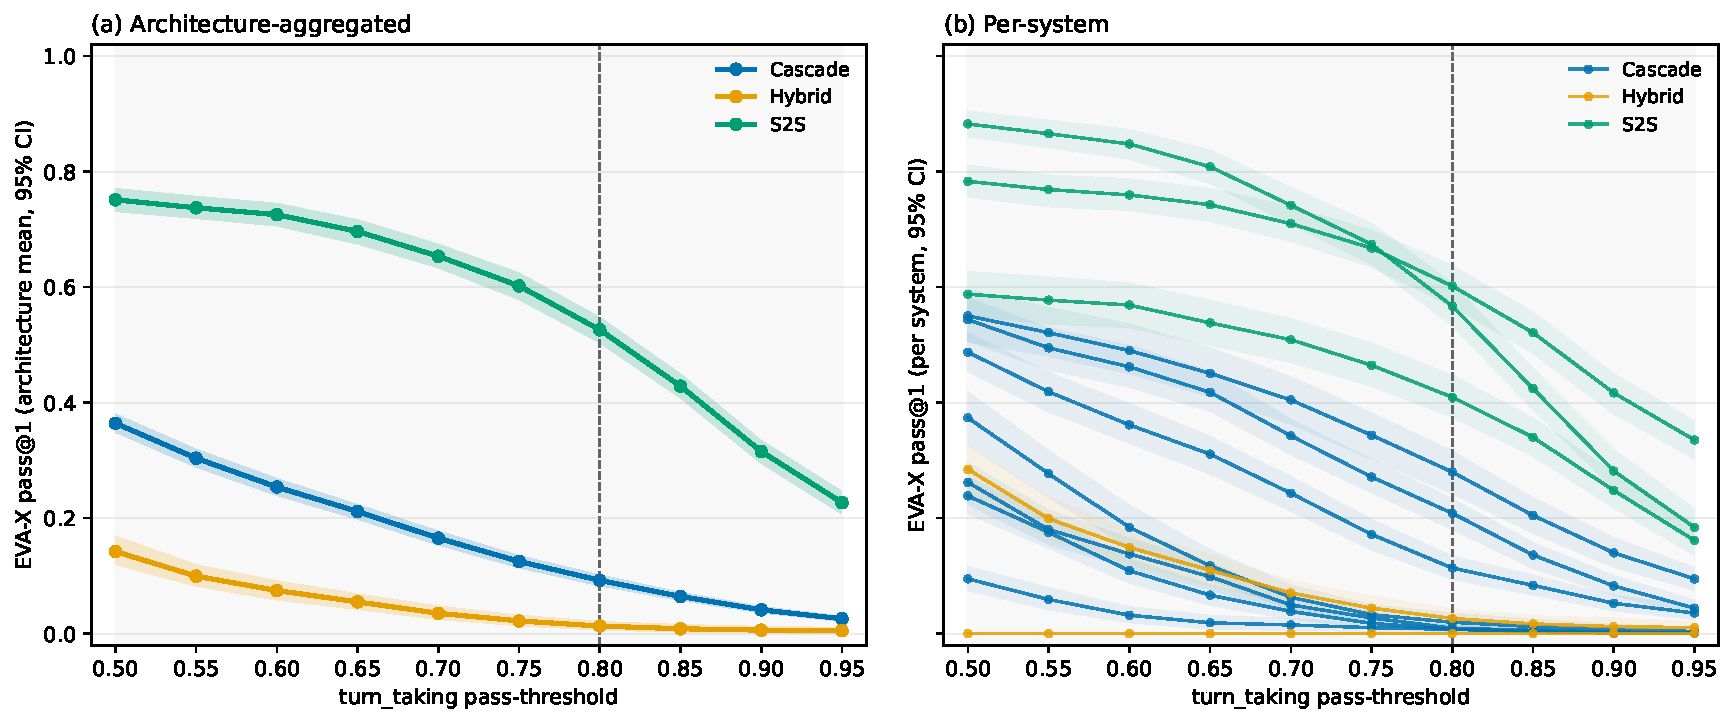
\includegraphics[width=\textwidth]{figures/threshold_sensitivity/threshold_sensitivity.pdf}
    \captionsetup{font=small}
    \caption{Sensitivity of EVA-X pass@1 to the turn-taking pass-threshold $\tau_{\text{tt}}$. We sweep $\tau_{\text{tt}}$ from $0.50$ to $0.95$ in $0.05$ increments and recompute EVA-X pass@1 at each value, holding the \metricconversationprogression~and \metricconcise~thresholds fixed at $0.5$. The dashed vertical line marks the pass threshold value $\tau_{\text{tt}} = 0.8$. (a) Architecture-aggregated. Each curve is the mean  per-scenario EVA-X pass@1 (averaged over $k = 5$ trials per scenario), pooled with equal weight across all (system, scenario) pairs within an architecture class (cascade, hybrid, S2S); shaded bands are  percentile bootstrap $95\%$ CIs from $1{,}000$ resamples of (system, scenario) pairs. (b) Per-system. One curve per benchmarked system, colored by architecture; shaded bands are bootstrap $95\%$ CIs from $1{,}000$ resamples of scenarios within the system. Architecture ordering (S2S > cascade > hybrid) is preserved at every threshold; per-system rankings flip only between close competitors.}
    \label{fig:threshold_sensitivity}
\end{figure*}

\paragraph{Why $\boldsymbol{0.8}$?}
The sensitivity sweep confirms that neither plateau nor cliff appears at any
candidate threshold. More importantly, the $0.23$-point gap between the highest
non-S2S system and the lowest S2S system means that any
$\tau_{\text{tt}} \in [0.6, 0.8]$ yields similar pass/fail assignments for
all 12 systems. We select the top of this range for two reasons:
(i)~it maps cleanly to the ``$4/5$ turns on-time'' interpretation, and
(ii)~it avoids compounding two layers of leniency, given that the on-time
bracket itself already extends beyond natural human turn-taking latency.
A higher threshold (e.g., $0.9$) is currently miscalibrated to model
capability---no system in our pool would reliably qualify.

\paragraph{Modularity and forward compatibility.}
EVA exposes \texttt{pass\_at\_k\_threshold} as a configurable metric parameter, and
practitioners benchmarking different system classes are encouraged to override the
default. The $0.8$ value reflects 2026 model capability; we expect this default to rise
as model latencies improve. The defense above is therefore a statement about the
\emph{current} calibration, not a fixed property of the metric.

\subsection{Diagnostic Metrics}
\label{app:diagnostic-metrics}
Diagnostic metrics include: \textit{Authentication Success Rate} (deterministic), \textit{Response Latency} in seconds decomposed into turns with and without tool calls or not (deterministic), speakability — whether agent text is voice-friendly prior to synthesis (LLM-as-Judge), STT word error rate computed via \texttt{jiwer} (deterministic), tool call validity — the fraction of tool calls with correctly formatted parameters (deterministic), and transcription accuracy for key entities — STT accuracy specifically on named entities such as names, dates, and alphanumeric codes (LLM-as-Judge). Together these metrics allow practitioners to distinguish, for example, between a task completion failure caused by an STT transcription error on a confirmation code versus one caused by incorrect LLM reasoning.
